\documentclass[11pt, a4paper, titlepage, openright]{article}

\usepackage{amsmath}
\usepackage[font=small,labelfont=bf]{caption}
\usepackage{float}
\restylefloat{figure}
\usepackage{graphicx}
\usepackage{hyperref}
\usepackage{mathtools}
\usepackage[titletoc, title]{appendix}
\usepackage{listings}
\usepackage{color}
\usepackage{fixltx2e}
\usepackage[bottom]{footmisc}

\definecolor{dkgreen}{rgb}{0,0.6,0}
\definecolor{gray}{rgb}{0.5,0.5,0.5}
\definecolor{mauve}{rgb}{0.58,0,0.82}

\lstset{frame=tb,
  language=C++,
  aboveskip=3mm,
  belowskip=3mm,
  showstringspaces=false,
  columns=flexible,
  basicstyle={\footnotesize\ttfamily},
  numbers=none,
  numberstyle=\tiny\color{gray},
  keywordstyle=\color{blue},
  commentstyle=\color{dkgreen},
  stringstyle=\color{mauve},
  breaklines=true,
  breakatwhitespace=true,
  tabsize=3,
  showstringspaces=false,
  keepspaces=true, 
  columns=flexible
}

\begin{document}
%%%%%%%%%%%%%%%%%%%%%%%%%%%%%%%%%%%%%%%%%
% University Assignment Title Page
% LaTeX Template
% Version 1.0 (27/12/12)
%
% This template has been downloaded from:
% http://www.LaTeXTemplates.com
%
% Original author:
% WikiBooks (http://en.wikibooks.org/wiki/LaTeX/Title_Creation)
%
% License:
% CC BY-NC-SA 3.0 (http://creativecommons.org/licenses/by-nc-sa/3.0/)
%
% Instructions for using this template:
% This title page is capable of being compiled as is. This is not useful for
% including it in another document. To do this, you have two options:
%
% 1) Copy/paste everything between \begin{document} and \end{document}
% starting at \begin{titlepage} and paste this into another LaTeX file where you
% want your title page.
% OR
% 2) Remove everything outside the \begin{titlepage} and \end{titlepage} and
% move this file to the same directory as the LaTeX file you wish to add it to.
% Then add \input{./title_page_1.tex} to your LaTeX file where you want your
% title page.
%
%%%%%%%%%%%%%%%%%%%%%%%%%%%%%%%%%%%%%%%%%

%----------------------------------------------------------------------------------------
%	PACKAGES AND OTHER DOCUMENT CONFIGURATIONS
%----------------------------------------------------------------------------------------
\begin{titlepage}

\newcommand{\HRule}{\rule{\linewidth}{0.5mm}} % Defines a new command for the horizontal lines, change thickness here

\center % Center everything on the page

%----------------------------------------------------------------------------------------
%	HEADING SECTIONS
%----------------------------------------------------------------------------------------

\textsc{\LARGE University of Antwerp}\\[1.5cm] % Name of your university/college
\textsc{\Large }\\[4cm] % Major heading such as course name
\textsc{\Large Scientific Programming}\\[0.5cm] % Minor heading such as course title

%----------------------------------------------------------------------------------------
%	TITLE SECTION
%----------------------------------------------------------------------------------------

\HRule
{ \huge \bfseries Second Session \\ \Large{Exercise 2}}\\ % Title of your document
\HRule \\[1.5cm]

%----------------------------------------------------------------------------------------
%	AUTHOR SECTION
%----------------------------------------------------------------------------------------

\begin{minipage}{0.4\textwidth}
\begin{flushleft} \large
Armin Halilovic - s0122210 % Your name
\end{flushleft}
\end{minipage}
~
\begin{minipage}{0.4\textwidth}
\begin{flushright} \large
\end{flushright}
\end{minipage}\\[4cm]

% If you don't want a supervisor, uncomment the two lines below and remove the section above
%\Large \emph{Author:}\\
%John \textsc{Smith}\\[3cm] % Your name

%----------------------------------------------------------------------------------------
%	DATE SECTION
%----------------------------------------------------------------------------------------

\vfill % Fill the rest of the page with whitespace
{\large August 22, 2016}\\[3cm] % Date, change the \today to a set date if you want to be precise

%----------------------------------------------------------------------------------------
%	LOGO SECTION
%----------------------------------------------------------------------------------------

%\includegraphics{Logo}\\[1cm] % Include a department/university logo - this will require the graphicx package

%----------------------------------------------------------------------------------------


\end{titlepage}
\tableofcontents
\newpage

\section{Problem}
    We are given the following set of data function:
    \[ f(x) = \sqrt{1 + \frac{x}{5}},\ where \ x \ \epsilon \ [-1, 1]\]

    We will approximate this function using fourier method:
    \[ g(t) = \frac{a_0}{2} + a_1 \cos (t) + a_2 \cos(2t) + ... + a_n \cos(nt) + b_1 \sin (t) + b_2 \sin (2t) + ... + b_m \sin (nt) \]


    This will be done using C++ and the \href{http://www.gnu.org/software/gsl/}{GNU Scientific Library}.
    In section~\ref{sec:solutions}, we will describe how we reached each solution, using the 
    most important parts from the code.

\bigskip
\bigskip
\section{Using the program}
    All of the C++ code for the program can be found in the main.cpp and in appendix A of this document.
    main.cpp comes accompanied by \mbox{function\_approximation.sh}, which contains all of the necessary UNIX commands to generate the graph images.
    This file relies on the \href{https://www.gnu.org/software/plotutils/manual/en/html_node/graph.html}{graph} program
    in the GNU plotutils package to plot graphs, so make sure that it is installed.

    To compile and run the program, execute the following commands in the build/ directory:
\begin{lstlisting}
cmake ..
make
chmod +x ./function_approximation.sh
./function_approximation.bin
\end{lstlisting}
    Do not forget the .bin extension. All of the graphs will be present in the build/images/ directory. If no graphs are present, they can be generated
    manually by executing function\_approximation.sh. \\
    Output files which give some extra information about the solutions can be found in console output  and appendix B.1.
    
\newpage
\section{Solutions}
\label{sec:solutions}
    In these solutions, m denotes the amount of data points we will use to approximate \( f(x) \) with.
    \subsection{Calculating the data points}
    We will generate m equidistant data points in the interval \([-1, 1]\), using the formula \( -1 + \frac{2*(i-1)}{m} \).  \\
    The array \(t\) will hold these points, array \(x\) will hold \( f(t) \). The points \(t_i\) wil then be rescaled to lie in \( [-\pi, \pi] \):
\begin{lstlisting}
double t[m], x[m];

for (int i = 1; i <= m; i++) {
    t[i-1] = -1 + (2*(i-1) / (double) (m-1));
    x[i-1] = fx(t[i-1]);
    t[i-1] = M_PI * t[i-1];
}
\end{lstlisting}
    \subsection{Calculating the coefficients}
    To use the approximating formula, we first need to find the coefficients \( a_0, a_1, b_1, a_2, b_2, ... \).
    The formulas for the coefficients are:
    \[ a_j = \frac{2}{m} \sum_{k=0}^{m-1}x_k \cos(j*t_k),\ \  b_j = \frac{2}{m} \sum_{k=0}^{m-1}x_k \sin(j*t_k) \]
    where \( j = 0, ..., n \) and \( x_k \) are the given data points we work with.
    In the code, this is done by the function "calcCoeff":
\begin{lstlisting}
double calcCoeff(double *t, double *x, bool a, int j, int m) {
    double result = 0;

    for (int k = 0; k < m; k++) {
        result += x[k] * ((a) ? gsl_sf_cos(j*t[k]) : gsl_sf_sin(j*t[k]));
    }

    result *= 2.0/(double) m;
    return result;
}
\end{lstlisting}
    \newpage
    \subsection{Approximating the function}
    We can now fill in and use the function
    \[ g(t) = \frac{a_0}{2} + a_1 \cos (t) + a_2 \cos(2t) + ... + a_n \cos(nt) + b_1 \sin (t) + b_2 \sin (2t) + ... + b_m \sin (nt) \]
    to approximate \(f(x)\):
    \\
\begin{lstlisting}
for (double t = -M_PI; t < M_PI; t = t + 0.01) {
    double y = coeff[0]; //y = a_0/2
    for (int i = 0; i < n; i++) {
        int j = 2*i+1;
        y += coeff[j]   * gsl_sf_cos((i+1)*t);
        y += coeff[j+1] * gsl_sf_sin((i+1)*t);
    }
}
\end{lstlisting}
    
    The approximation functions \( f(t) \) can be found in Appendix B.1. 
    The graphs that are generated can be found in Appendix B.2 and B.3. The graphs in Appendix B.3 are approximations for \( f(x) = |x| \).
    
    We notice in both cases that, generally, the approximation becomes more accurate with an increase in m or n. This is to be expected with fourier methods.

\onecolumn
\appendix
\appendixpage
\addappheadtotoc

\section{Code}
	\subsection{main.cpp}
		\lstinputlisting[basicstyle=\scriptsize]{../main.cpp}
	\bigskip
	\subsection{function\_approximation.sh}
		\lstinputlisting[basicstyle=\scriptsize, language=bash]{../build/function_approximation.sh}

\newpage
\section{Output}
\label{sec:output}
	\subsection{Console output}
	\label{sec:consoleOut}
		\lstinputlisting[basicstyle=\scriptsize]{../consoleOutput.txt}

	\subsection{\( f(x) = \sqrt{1 + \frac{x}{5}} \)}
	\label{sec:sqrtImages}
    \begin{figure}[H]
        \begin{minipage}[b]{0.49\textwidth}
            \includegraphics[width=6.5cm, trim={2cm, 4cm, 2cm, 3cm}, clip]{../build/images/fx}
        \end{minipage}
        \hfill
        \begin{minipage}[b]{0.49\textwidth}
            \includegraphics[width=6.5cm, trim={2cm, 4cm, 2cm, 3cm}, clip]{../build/images/m3n1}
        \end{minipage}
        \caption{left: f(x), right: approximation where m=3 and n=1}
        \label{fig:sqrt1}
    \end{figure}
    \begin{figure}[H]
        \begin{minipage}[b]{0.49\textwidth}
            \includegraphics[width=6.5cm, trim={2cm, 4cm, 2cm, 3cm}, clip]{../build/images/m5n1}
        \end{minipage}
        \hfill
        \begin{minipage}[b]{0.49\textwidth}
            \includegraphics[width=6.5cm, trim={2cm, 4cm, 2cm, 3cm}, clip]{../build/images/m10n1}
        \end{minipage}
        \caption{approximations where m=5, n=1, and m=10, n=1}
        \label{fig:sqrt1}
    \end{figure}
    \begin{figure}[H]
        \begin{minipage}[b]{0.49\textwidth}
            \includegraphics[width=6.5cm, trim={2cm, 4cm, 2cm, 3cm}, clip]{../build/images/m25n1}
        \end{minipage}
        \hfill
        \begin{minipage}[b]{0.49\textwidth}
            \includegraphics[width=6.5cm, trim={2cm, 4cm, 2cm, 3cm}, clip]{../build/images/m3n3}
        \end{minipage}
        \caption{approximations where m=25, n=1, and m=3, n=3}
        \label{fig:sqrt1}
    \end{figure}
    \begin{figure}[H]
        \begin{minipage}[b]{0.49\textwidth}
            \includegraphics[width=6.5cm, trim={2cm, 4cm, 2cm, 3cm}, clip]{../build/images/m5n3}
        \end{minipage}
        \hfill
        \begin{minipage}[b]{0.49\textwidth}
            \includegraphics[width=6.5cm, trim={2cm, 4cm, 2cm, 3cm}, clip]{../build/images/m10n3}
        \end{minipage}
        \caption{approximations where m=5, n=3, and m=10, n=3}
        \label{fig:sqrt1}
    \end{figure}
    \begin{figure}[H]
        \begin{minipage}[b]{0.49\textwidth}
            \includegraphics[width=6.5cm, trim={2cm, 4cm, 2cm, 3cm}, clip]{../build/images/m25n3}
        \end{minipage}
        \hfill
        \caption{approximation where m=25, n=3}
        \label{fig:sqrt1}
    \end{figure}
    
    \bigskip
    \bigskip
    \bigskip
    \bigskip
	\subsection{Extra: \( f(x) = |x| \)}
	\label{sec:absImages}
    \begin{figure}[H]
        \begin{minipage}[b]{0.49\textwidth}
            \includegraphics[width=6.5cm, trim={2cm, 4cm, 2cm, 3cm}, clip]{../absImages/fx}
        \end{minipage}
        \hfill
        \begin{minipage}[b]{0.49\textwidth}
            \includegraphics[width=6.5cm, trim={2cm, 4cm, 2cm, 3cm}, clip]{../absImages/m3n1}
        \end{minipage}
    \end{figure}
    \begin{figure}[H]
        \begin{minipage}[b]{0.49\textwidth}
            \includegraphics[width=6.5cm, trim={2cm, 4cm, 2cm, 3cm}, clip]{../absImages/m5n1}
        \end{minipage}
        \hfill
        \begin{minipage}[b]{0.49\textwidth}
            \includegraphics[width=6.5cm, trim={2cm, 4cm, 2cm, 3cm}, clip]{../absImages/m10n1}
        \end{minipage}
    \end{figure}
    \begin{figure}[H]
        \begin{minipage}[b]{0.49\textwidth}
            \includegraphics[width=6.5cm, trim={2cm, 4cm, 2cm, 3cm}, clip]{../absImages/m25n1}
        \end{minipage}
        \hfill
        \begin{minipage}[b]{0.49\textwidth}
            \includegraphics[width=6.5cm, trim={2cm, 4cm, 2cm, 3cm}, clip]{../absImages/m3n3}
        \end{minipage}
    \end{figure}
    \begin{figure}[H]
        \begin{minipage}[b]{0.49\textwidth}
            \includegraphics[width=6.5cm, trim={2cm, 4cm, 2cm, 3cm}, clip]{../absImages/m5n3}
        \end{minipage}
        \hfill
        \begin{minipage}[b]{0.49\textwidth}
            \includegraphics[width=6.5cm, trim={2cm, 4cm, 2cm, 3cm}, clip]{../absImages/m10n3}
        \end{minipage}
    \end{figure}
    \begin{figure}[H]
        \begin{minipage}[b]{0.49\textwidth}
            \includegraphics[width=6.5cm, trim={2cm, 4cm, 2cm, 3cm}, clip]{../absImages/m25n3}
        \end{minipage}
        \hfill
    \end{figure}

\end{document}